\documentclass{beamer}

\usetheme{metropolis}
\usecolortheme{metropolis}
\usepackage{fontspec}
\usepackage{mathtools}
\usepackage{graphicx}
\usepackage{listings}
\usepackage{pdfpages}

\setmainfont{Times New Roman}
\setsansfont{Arial}
\setmonofont{Courier New}

\lstset{language=[Sharp]C,
        basicstyle=\ttfamily\scriptsize,
        breaklines=true}

\title{Задача развоза продуктов}

\date{2018}

\begin{document}
\frame{\titlepage}
\begin{frame}
    \begin{figure}
        \centering
        Первая презентация
    \end{figure}
\end{frame}
\setbeamercolor{background canvas}{bg=}

\includepdf[pages=2-7]{1_pres.pdf}
\begin{frame}
    \begin{figure}
        Вторая презентация
    \end{figure}
\end{frame}

\includepdf[pages=2-12]{2_pres.pdf}
\begin{frame}
    \begin{figure}
        Третья презентация
    \end{figure}
\end{frame}
\begin{frame}
    \frametitle{Постановка задачи}
    Дан город, на котором отмечены разные пункты, среди которых есть магазины и склад.
    Заранее оговорённое количество машин должно развести продукты по магазинам со склада
    таким образом, чтобы максимальная длина пути среди каждой машины была минимальной.
\end{frame}
\begin{frame}
    \frametitle{Математическая модель}
    Дано:
    Граф \( G = (V, E) \), где V - множество пунктов, а E - 
    множество дорог\\*
    \(n\) - количество пунктов\\*
    \(m\) - количество магазинов\\*
    \(k\) - количество машин\\*
    \(S\) - склад\\*
    \(M = \{M_1, ..., M_m\}\) - множество магазинов (сочетание из n 
    по m множества V)\\
    Промежуточные данные:\\*
    \(d[i, j]\) - длина кратчайшего пути между магазинами i и j.\\*
    \(ds[i]\) - длина кратчайшего пути от склада до магазина i
\end{frame}
\begin{frame}
    \frametitle{Математическая модель}
    Нужно найти:\\*
    \(c_i = (c_{i,1}, ..., c_{i,r_i})\) - размещение 
    из \(m\) по \(r_i\) множества \(M\) - множество пунктов,
    которое охватывает \(i\)-я машина, где \(r_i\) - количество магазинов, которые проезжает \(i\)-я машина.\\
    Целевая функция:
    \[\max_{1 \leq i \leq k} \left(ds[c_{i,1}] + \sum\limits_{j = 2}^{r_i}d[c_{i,j-1}][c_{i,j}] + ds[c_{i,r_i}]\right) \longrightarrow min \]
\end{frame}
\begin{frame}
    \frametitle{Алгоритм}
    При решении задачи был реализован генетический алгоритм. Для этого требовалось
    закодировать подходящим образом решения и разработать функции, которые
    определяют поведение алгоритма: генерация первичной популяции, мутация, скрещивание и селекция.
\end{frame}
\begin{frame}
    \frametitle{Кодирование}
    Для манипуляций с решениями они были представлены в следующем виде:
    Каждая особь содержит два массива - массив всех магазинов, расположенных
    в определенном порядке, и массив машин. В массиве машин в i-й ячейке находится
    число магазинов, которые проезжает i-я машина. Обозначим это число за \(k_i\).
    Магазины же расположены таким образом, что первые \(k_1\) магазинов проезжает
    1-я машина, после идут \(k_2\) магазинов, которые проезжает вторая машина и т.д.
\end{frame}
\begin{frame}
    \frametitle{Кодирование}
    Пример:
    \begin{center}
        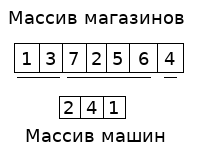
\includegraphics[height=4cm]{encoding.png}
    \end{center}
\end{frame}
\begin{frame}
    \frametitle{Генерация первичной популяции}
    Первичная популяция состоит из одной особи и генерируется
    случайным образом. 
    Генерация массива магазинов у особи проста: обходом ячеек подряд
    записываем них случайный еще не посещенный магазин.
    Генерация массива машин: генерируется количество посещяемых
    магазинов среди свободных и присваивается случайной машине.
    Генерируемое количество гарантирует, что как минимум 2 магазина
    достанется каждой машине. Последней машине достаются все оставшиеся
    магазины.
\end{frame}
\begin{frame}
    \frametitle{Мутация}
    Используется 2 вида мутации.\\*
    Первая мутация - в массиве магазинов у особи меняются местами два магазина.\\*
    Вторая мутация - у одной машины уменьшается длина пути на случайное число, у другой машины увеличивается на это же число.
    На каждую особь может быть применена либо первая, либо вторая мутация. Исходная особь сохраняется.
\end{frame}
\begin{frame}
    \frametitle{Скрещивание}
    Скрещивание определено следующим образом:\\*
    Берутся случайные родители из популяции, затем у первого родителя
    из массива магазинов выделяется последовательность, и она
    переносится в рёбенка. Затем те магазины, которых недостаёт в 
    ребенке, берутся из второго родителя, в том порядке, в котором они у 
    него встречаются.
\end{frame}
\begin{frame}
    \frametitle{Скрещивание}
    Пример:
    
    \begin{center}
        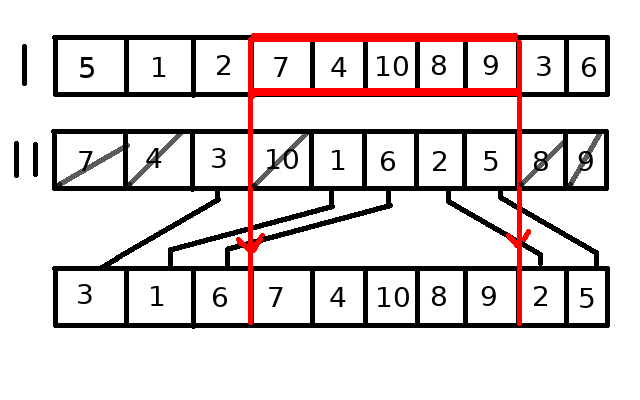
\includegraphics[height=6cm]{crossover.png}
    \end{center}
\end{frame}
\begin{frame}
    \frametitle{Селекция}
    В данном алгоритме применена турнирная селекция:\\*
    Вся популяция делится на группы, и среди каждой группы
    выживают только особи с наилучшим значением целевой функции.
\end{frame}
\begin{frame}
    \frametitle{Структура программы}
    Программа состоит из несколько классов:\\*
    Класс \textbf{Products}, который отвечает за чтение данных и
    трансформацию изначального графа в полный. Он передаёт эти данные
    объекту класса
    \textbf{MtspSolver}, в котором определены методы
    \textit{Selection}, \textit{Mutation},
    \textit{Crossover} и \textit{Solve}, с помощью которого и запускается алгоритм.
    В классе \textbf{MtspSolver} определены константы: количество
    особей в первичной популяции, количество мутаций и количество
    скрещиваний. \\*
    Также есть класс \textbf{Solution}, который является классом особей.
    Он определяет полезные методы для копирования особей, получения 
    их массивов, итерирования и представления особи в виде строки.
\end{frame}
\begin{frame}
    \frametitle{Формат входного файла}
    Входной файл подаётся в следующем формате:\\
    Первая строка: <количество машин> <склад>\\
    Вторая строка: перечисление магазинов через пробел\\
    На каждой следующей строке расположено 3 числа через пробел:
    Первая вершина, вторая вершина и вес ребра между ними
\end{frame}
\begin{frame}
    \frametitle{Время работы}
    Алгоритм был протестирован на графе с около 80 тысячами рёбер и 200 магазинами.
    Примерно за минуту достигается результат, который хуже оптимального на 20\%.
    При продолжении работы алгоритм способен максимально приблизиться к оптимальному решению.
\end{frame}
\begin{frame}[fragile]
\frametitle{Класс Products}
\lstinputlisting{Products.src}
\end{frame}
\begin{frame}[fragile]
\frametitle{Класс MtspSolver}
\lstinputlisting[firstline=1, lastline=14]{Solve.src}
\end{frame}
\begin{frame}[fragile]
\lstinputlisting[firstline=15]{Solve.src}
\end{frame}
\begin{frame}
\frametitle{Участники}
\begin{itemize}
    \item Саблина Анастасия
    \item Садукова Анастасия
    \item Карповский Денис
    \item Кононов Кирилл
\end{itemize}
\end{frame}
\end{document}
